\documentclass[12pt]{article}
\usepackage{bm}
\usepackage{graphicx}
\usepackage{gensymb}
\usepackage{float}
\usepackage[a4paper, total={6in, 8in}]{geometry}

\graphicspath{{./../images/}}

\begin{titlepage}

\title{\textbf{Optimum Loft Angle for Greatest Carry Distance}}
\author{\textbf{Group D}\\
		Alison McIntosh\\
		Emily Dark\\
		Henry Archer\\
		Kyle Stewart\\
		Stuart Ballantyne}
\date{}

\end{titlepage}

\begin{document}

\begin{titlepage}
\maketitle
\thispagestyle{empty}
\pagebreak
\end{titlepage}

\pagenumbering{arabic}

\section{Abstract}
...


\section{Response}
...

\section{Theory and model}

\subsection{Assumptions}
The following assumptions are made throughout the report and model:
\begin{description}
  \item[$\cdot$] golf course is level and has no effect on trajectory;
  \item[$\cdot$] height of the tee is negligible;
  \item[$\cdot$] gravitational field strength is constant (9.81 $N\cdot kg^{-1}$) and does not flucuate with height;
  \item[$\cdot$] driver is roughly a flat plate and strikes the ball precisely at the center, with no draw or fade;
  \item[$\cdot$] the ball used is a Titleist Pro V1, with a mass of $45.93$ g, diameter of $42.67$ mm.
  	
\end{description}

\subsection{Impact}
...
\pagebreak
\subsection{Flight}
\subsubsection{Simple golf ball}
A simple golf ball experiencing only weight may be modelled by the following system of differential equations;
\begin{equation}
a_x=\frac{\partial v_x}{\partial t}=0
\end{equation}
\begin{equation}
a_y=\frac{\partial v_y}{\partial t}=-g
\end{equation}
where $g$ is the gravitional field strength.

Assuming the initial velocity is $v_0$ and the launch angle is $\theta$, the above equations can be solved to give:
\begin{equation}
v_x=v_0 \cos{\theta}
\end{equation}
\begin{equation}
v_y=v_0 \sin{\theta}-gt
\end{equation}
Integrating the above equations with respect to time gives the displacement as a function of time:
\begin{equation}
x=v_0 t \cos{\theta}
\end{equation}
\begin{equation}
y=v_0 t \sin{\theta}-\frac{1}{2} g t^2
\end{equation}

The maximum range is achieved when

\begin{figure}[H]
\centering
\caption{Golf ball trajectory under no air resistance or lift}
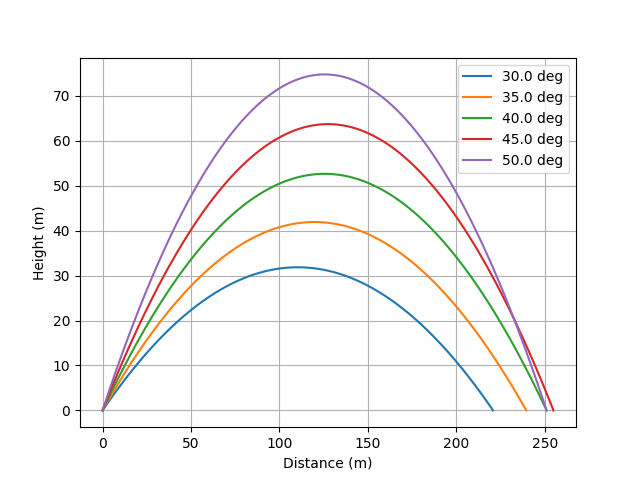
\includegraphics[scale=0.7]{simple}
\end{figure}

\begin{figure}[H]
\centering
\caption{Range as a function of loft angle, no drag or lift}
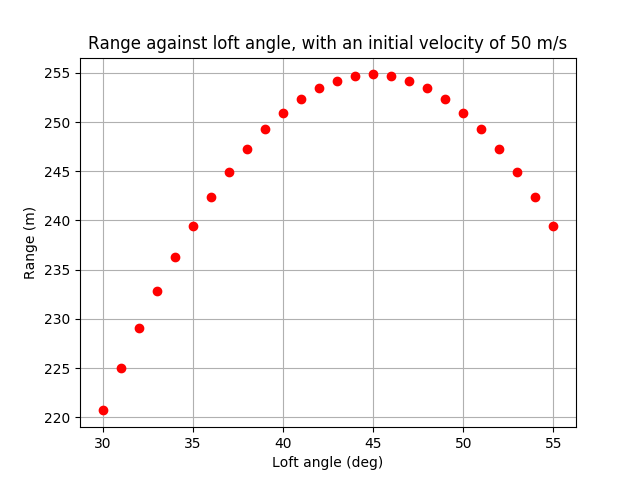
\includegraphics[scale=0.8]{simplerange}
\end{figure}

Figures (1) and (2) show the maximum range is when the loft angle at 45\degree, as predicted by the equations of projectile motion.
\pagebreak
\subsubsection{Smooth golf ball experiencing drag}
The drag equation is:
\begin{equation}
\vec{F_d} = \frac{1}{2} A C_d \rho_{air} |\vec{v}| \vec{v}
\end{equation}
where $\rho_{air}$ is the density of air; $A$ is the reference area, which in the case of a smooth sphere of radius $r$, is the cross-sectional area $\pi r^2$; $C_d$ is the coefficient of drag, which is dependent on the Reynolds number; and $\vec{v}$ is the flow velocity relative to the golf ball.

Applying equation (7) to equations (1)-(2), we get
\begin{equation}
\frac{\partial v_x}{\partial t}=-k |v_x| v_x
\end{equation}
\begin{equation}
\frac{\partial v_y}{\partial t}=-g-k |v_y| v_y
\end{equation}
where $k=\frac{1}{2} A C_d \rho$.
\begin{figure}[H]
\centering
-\caption{Golf ball trajectory when experiencing drag but no lift, $C_d=0.5$}
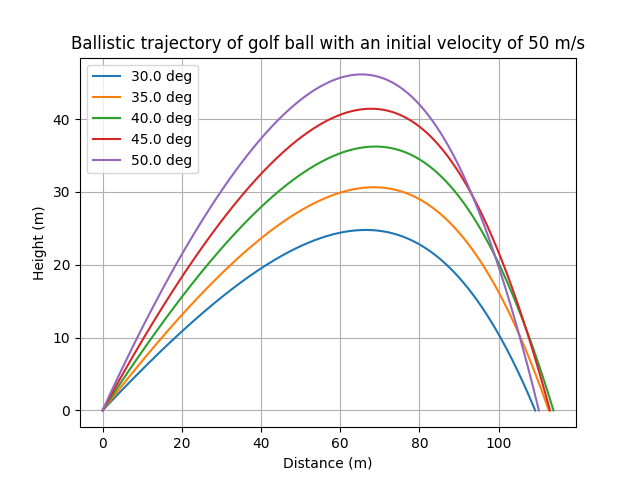
\includegraphics[scale=0.85]{dragapprox}
\end{figure}

\begin{figure}[H]
\centering
\caption{Range as a function of loft angle, $C_d$ = 0.5}
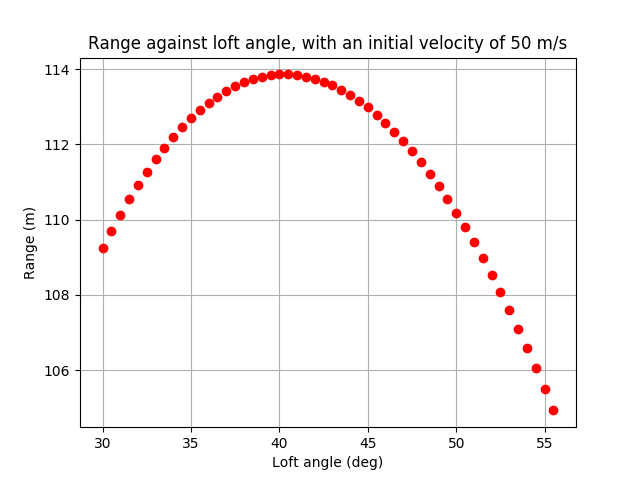
\includegraphics[scale=0.9]{dragapproxrange}
\end{figure}

Figure (4) shows that the maximum range is achieved at 40.2\degree, for an initial velocity of $50$ $m\cdot s^{-1}$. Additionally, the range is significantly decreased when drag was added to the model. The greatest range with drag is about $114$ m versus the previous range of $255$ m at 45.0\degree.
However, $C_d$ is not constant and depends on the Reynolds number, which is proportional to the velocity of the golf ball. The Reynolds number is given by:
\begin{equation}
Re=\frac{2vr}{\nu}
\end{equation}
where $\nu$ is the kinematic viscosity of air.

Using data from [whereever we found the Reynolds number data], we used Python to find a fourth-order polynomial approximation as shown in Figure (5).

\begin{figure}[H]
\centering
\caption{Coefficient of drag as a function of Reynolds number with curve of best fit}
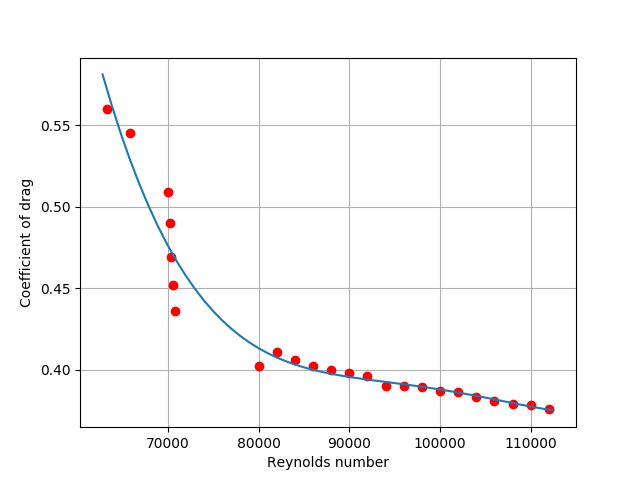
\includegraphics[scale=0.85]{reynolds}
\end{figure}

Applying the polynomial approxmation for the coefficient of drag and equation (10), the optimum loft angle decreases down to about 34.5\degree, shown in figures (6)-(7).
\begin{figure}[H]
\centering
\caption{Trajectory of golf ball with drag considering Reynolds number, $v_i=50 m\cdot s^{-1}$}
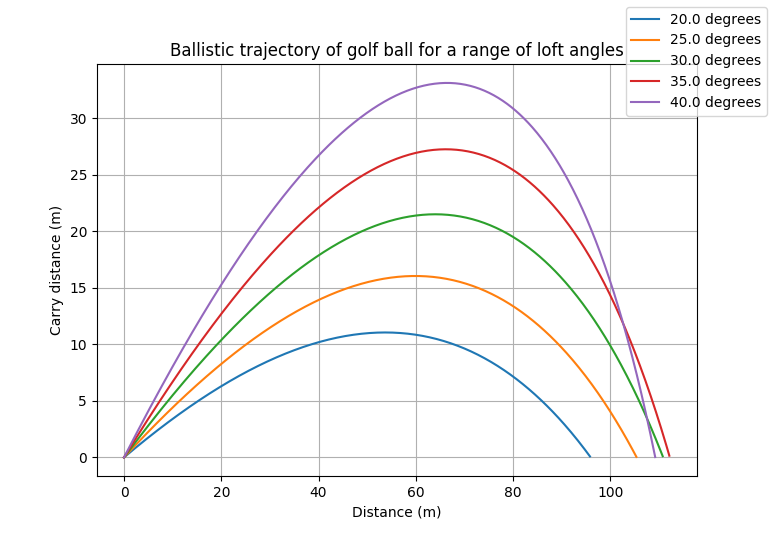
\includegraphics[scale=0.65]{dragwithreynolds}
\end{figure}

\begin{figure}[H]
\centering
\caption{Range against loft angle for golf ball with drag considering Reynolds number, $v_i=50 m\cdot s^{-1}$}
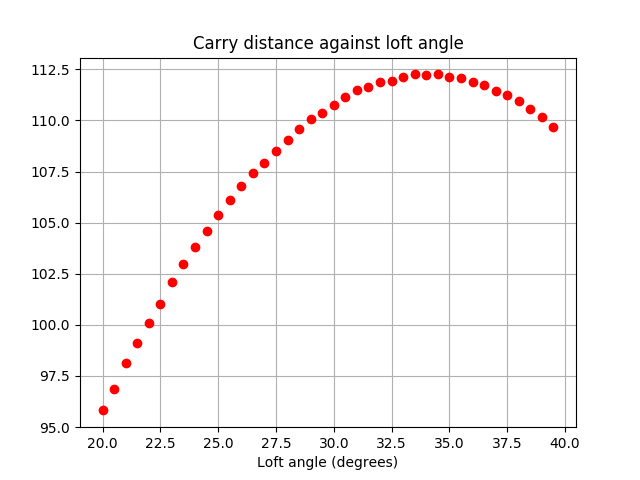
\includegraphics[scale=0.7]{dragwithreynoldsrange}
\end{figure}

\end{document}
\grid